\documentclass[12pt]{article}


\usepackage{tikz}
\usetikzlibrary{calc}

\begin{document}

\def\vertexLabels{true}

            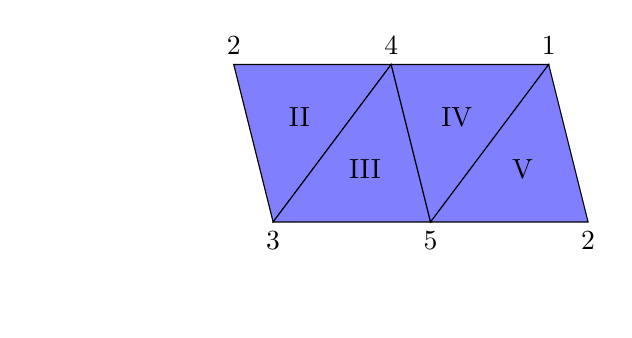
\begin{tikzpicture}
                \coordinate [label=below:\if \vertexLabels 1 \fi] (A) at (0,0);
                \coordinate [label=above:2] (B) at (1.5,2);
                \coordinate [label=below:3] (C) at (2,0);
                \coordinate [label=above:4] (D) at ($(B)+(C)$);
                \coordinate [label=below:5] (E) at ($2*(C)$);
                \coordinate [label=above:1] (F) at ($2*(C)+(B)$);
                \coordinate [label=below:2] (G) at ($3*(C)$);

                % Draw a face with vertices 1,2,3 and label 4 in the middle
                \def\drawFace#1#2#3#4{
                    \filldraw[fill=blue!50!white, draw=black] (#1) -- (#2) -- (#3) -- cycle;
                    \node at ($1/3*(#1)+1/3*(#2)+1/3*(#3)$) {#4};
                }
                
                \node at (-1,-1) {\vertexLabels};
                
			\ifx \vertexLabels = true
                \drawFace{A}{B}{C}{I}
            \fi
                \drawFace{B}{C}{D}{II}
                \drawFace{C}{D}{E}{III}
                \drawFace{D}{E}{F}{IV}
                \drawFace{E}{F}{G}{V}
            \end{tikzpicture}
\end{document}